%!TEX root = ../thesis.tex
%*******************************************************************************
%*********************************** Statistics *********
%*******************************************************************************


\chapter{Statistical data analysis}\label{ch:statistics}

\graphicspath{{chapter-statistics/Figs/Vector/}{chapter-statistics/Figs/}}

In \gls{hep}, statistical models are used in order to quantify the correspondence between theoretical predictions and the experimental observations.
This chapter introduces the statistical concepts, methods and formulae used for statistical inference in this thesis.
A frequentist approach is employed, interpreting probabilities as the frequencies of the outcomes of repeatable experiments that may either be real, based on computer simulations, or mathematical abstraction~\cite{pdg2020}.
The following description largely adheres to \references\cite{Cranmer:2015nia, Cowan:2010js}.

\section{The likelihood function}\label{sec:likelihood_function}
 
In measurements in \gls{hep}, a \textit{statistical model} $f(\makemebold{x}\vert\makemebold{\phi})$ is a parametric family of \glspl{pdf} describing the probability of observing data $\makemebold{x}$ given a set\footnote{Sets of parameters (as opposed to single parameters) will henceforth be written using bold face.} of model parameters $\makemebold{\phi}$.
The latter typically describe parameters of the physical theory or unknown detector effects. The \textit{likelihood function} $L(\makemebold{\phi})$ is then numerically equivalent to $f(\makemebold{x}\vert\makemebold{\phi})$ with $\makemebold{x}$ fixed.
As opposed to the \glsfirst{pdf} $f(\makemebold{x})$ describing the value of $f$ as a function of $\makemebold{x}$ given a set of fixed parameters $\makemebold{\phi}$, the likelihood refers to the value of $f$ as a function of $\makemebold{\phi}$ given a fixed\footnote{This important difference is why the likelihood is written here as $L(\makemebold{\phi})$ instead of the equally common $L(\makemebold{x}\vert\makemebold{\phi})$.} value of $\makemebold{x}$.

Searches for \gls{bsm} physics are often\footnote{While searches for \gls{bsm} physics using unbinned distributions also exist, only binned searches are considered in the following.} centred around the measurement of several disjoint binned distributions, called \textit{channels} $c$, each associated with different event selection criteria yielding observed event counts $\makemebold{n}$.
In such counting experiments where each event is independently drawn from the same underlying distribution, each bin is described by a Poisson term.
The Poisson probability to observe $n$ events with an expectation of $\nu$ events, $\mathrm{Pois}(n\vert\nu)$, is given by
\begin{equation}
	\mathrm{Pois}(n\vert\nu) = \frac{\nu^n}{n!}e^{-\nu}.
\end{equation}
The expectation $\nu_{cb}$ in each channel $c$ and bin $b$ is a sum over the set of physics processes considered, called \textit{samples} in the following, 
\begin{equation}
	\nu_{cb} = \sum_{s\in\mathrm{samples}}\nu_{csb}(\makemebold{\eta},\makemebold{\chi}),
\end{equation}
where $\nu_{csb}$ is the expected sample rate in a given bin of a given channel. The sample-wise rates are in general a function of the model parameters $\makemebold{\phi}$ that can either be \textit{free parameters} $\makemebold{\eta}$ or \textit{constrained parameters} $\makemebold{\chi}$. Possible modifications of the expected sample rates due to model parameters are considered to be either multiplicative or additive changes to the nominal estimate $\nu_{csb}^0$ of the form
\begin{equation}
	\nu_{csb}(\makemebold{\eta},\makemebold{\chi}) = \left(\prod_i f^i_{csb}(\makemebold{\eta},\makemebold{\chi}) \right)\left(\nu^0_{csb} + \sum_j {\Delta^j_{csb}(\makemebold{\eta},\makemebold{\chi})} \right).
\end{equation}
Here, $\makemebold{f}(\makemebold{\phi})$ and $\makemebold{\Delta}(\makemebold{\phi})$ are the multiplicative and additive \textit{rate modifiers}, respectively, modifying the nominal estimates. Although in practice often only a function of a single model parameter, the rate modifiers can in general be a function of a set of model parameters.

Free parameters directly determined by the data observations are called \textit{normalisation factors}.
The constrained parameters represent the systematic uncertainties considered in the model, which---in frequentist statistics---have fixed but unknown true values.
The degree to which they cause a deviation of the expected event rates from the nominal event rates is limited through \textit{constraint terms} $c_{\makemebold{\chi}}(a_{\makemebold{\chi}}\vert\makemebold{\chi})$ that can be viewed as \textit{auxiliary measurements} with global observed data $\makemebold{a}$. 

For a given observation $\makemebold{x} = (\makemebold{n},\makemebold{a})$ of observed events $\makemebold{n}$ and auxiliary data $\makemebold{a}$, the likelihood then reads
\begin{equation}
	L (\makemebold{\eta}, \makemebold{\chi}) = \prod_{c\in\mathrm{channels}} \prod_{b\in\mathrm{bins_c}} \mathrm{Pois}(n_{cb}\vert\nu_{cb}(\makemebold{\eta},\makemebold{\chi})) \prod_{\chi\in\makemebold{\chi}}c_\chi (a_\chi\vert\chi),
\end{equation}
where, given a certain integrated luminosity, $n_{cb}$ and $\nu_{cb}$ refer to the corresponding observed and expected rate of events, respectively~\cite{ATL-PHYS-PUB-2019-029}.
Most of the systematic uncertainties are so-called \textit{interpolation parameters} $\makemebold{\alpha}$ representing either normalisation uncertainties or correlated shape uncertainties\improvement{Explain this further}.
Their constraint terms $c_{\makemebold{\alpha}}(a_{\makemebold{\alpha}}\vert\makemebold{\alpha})$ are parametrised by a Gaussian\footnote{Other parameterisations are also possible and discussed in \reference\cite{Cranmer:1456844}, but not used in the following.} with mean $a = 0$ and variance $\sigma = 1$, with $\alpha = 0$ representing the nominal value.
The \textit{up} and \textit{down} variations are then given by $\alpha=\pm 1$, thereby representing $\pm 1\sigma$ variations.
The impact of any given value of the parameter on the event rates is subsequently evaluated through polynomial interpolation and exponential extrapolation\footnote{Different interpolation and extrapolation strategies are discussed in \reference\cite{Cranmer:1456844} but not mentioned herein as they will not be used in the following.}, a method that avoids discontinuous first and second derivatives at $\alpha = 0$ and ensures positive values for the predicted event rates~\cite{Cranmer:1456844}.

Sample rates derived directly from theory calculations (\ie \gls{mc} simulation), are scaled to the integrated luminosity corresponding to the observed data.
As discussed in~\cref{sec:lumi_datataking}, the integrated luminosity is itself a measurement that is subject to uncertainties, requiring an additional constraint term in the likelihood.
It is parametrised by a Gaussian with mean corresponding to the nominal integrated luminosity measurement and standard deviation equal to the integrated luminosity measurement uncertainty.
Uncertainties arising from the finite size of the \gls{mc} datasets used to derive estimated event rates are modelled by bin-wise scale factors $\gamma_b$.
The constraint terms are Gaussian distributions with central value equal to unity and standard deviations calculated from the individual uncertainties of the samples defined in the respective channel.

As the event rate in a given bin can depend on multiple parameters, and likewise, a single parameter can affect the expected event rate in multiple bins across various channels, correlations between the model parameters $\makemebold{\phi}$ can occur.

The above prescription for building binned likelihoods is called the \textsc{HistFactory} template~\cite{Cranmer:1456844}. In this work, two independent implementations of the \textsc{HistFactory} template are used.
The first implementation, predominantly used in~\cref{part:simplified_model_analysis}, relies on \textsc{RooFit}~\cite{RooFit:2003ir} (using the \texttt{Minuit}~\cite{James:310399} package) and \textsc{RooStats}~\cite{RooStats:2010pm} for model parameter estimation and hypothesis tests, and is fully integrated into the \textsc{Root} data analysis framework~\cite{ROOT:1997pa,ROOT-2}. The user interface and the steering of statistical fits, as well as the bookkeeping of their results, is provided by \textsc{HistFitter}~\cite{HistFitter:2014wma}.
The second implementation, used in~\cref{part:reinterpretation}, makes use of \texttt{pyhf}~\cite{pyhf_joss,pyhf}, a recent pure-\texttt{python} implementation of \textsc{HistFactory} that is independent of the \textsc{Root} environment.
The \texttt{pyhf} implementation of \textsc{HistFactory} relies on \textsc{Numpy}~\cite{numpy} and uses computational graph libraries like \textsc{PyTorch}~\cite{pytorch}, \textsc{TensorFlow}~\cite{tensorflow2015-whitepaper} and \textsc{JAX}~\cite{jax2018github} to significantly speed up the parameter estimation process by leveraging the computational advantages of tensor algebra and automatic differentiation.
 
Apart from separating the model parameter set into free and constrained parameters $\makemebold{\phi} = (\makemebold{\eta},\makemebold{\chi})$, a separate partition $\makemebold{\phi} = (\makemebold{\psi},\makemebold{\theta})$ is frequently used in the context of hypothesis testing.
Here, $\makemebold{\psi}$ are so-called \textit{parameters of interests} of the model for which hypothesis tests are performed, and $\makemebold{\theta}$ are \textit{nuisance parameters} that are not of immediate interest but need to be accounted for to correctly model the data.
In the search presented in this work, the only \gls{poi} is the \textit{signal strength} parameter $\mu$, representing the ratio of the signal process cross section to its reference cross section as expected from theory.
The expected event rate $\nu_i$ in each bin $i$ can then be parametrised through
\begin{equation}
	\nu_b = \mu S_b + B_b,
\end{equation}
where $S_b$ and $B_b$ are the bin-wise expected signal and background rates, respectively. Fixing $\mu = 0$ thus yields an expected event rate containing only \gls{sm} processes, which is why this is also called a \textit{background-only} configuration. Setting $\mu = 1$ represents a \textit{signal-plus-background} description at nominal signal cross section. Scanning multiple values of $\mu$ allows to set limits on the visible cross sections of the signal models considered in the search. 
  
\section{Parameter estimation}

Given a likelihood $L(\makemebold{\phi})$ for a fixed set of observations $\makemebold{x}$, a measurement can be understood as a parameter estimation. In general, an estimator $\hat{\phi}$ is a function of the observed data used to estimate the true value of the model parameter $\phi$.

In particle physics, the most commonly used estimator is the \gls{mle}. The \glspl{mle} for the model parameters $\makemebold{\hat{\phi}}$ are defined to be the parameter values that maximise $L(\makemebold{\phi})$, or equivalently, maximise $\ln{L(\makemebold{\phi})}$ and minimise $-\ln{L(\makemebold{\phi})}$. The logarithm of the likelihood is used for computational reasons, as it not only reduces the computational complexity by avoiding exponentials and products, but also avoids potential problems arising from finite floating point precision. As the logarithm is a monotonically increasing function, $\ln{L(\makemebold{\phi})}$ has maxima at the same parameter values as ${L(\makemebold{\phi})}$. The negative logarithm of the likelihood is chosen in order to stick to the convention of optimisers in statistical packages typically minimising the result of a \textit{loss function}.

The \glspl{mle} $\makemebold{\hat{\phi}}$ can thus be found by solving the system of equations
\begin{equation}
 \frac{\uppartial \ln L}{\uppartial\phi_i} = 0,
\end{equation}
where the index $i$ runs over all parameters. Due to the complexity of the likelihood, a solution typically needs to be found numerically using minimisation algorithms. In the following, the parameter estimation is referred to as a \textit{fit} of the model to data, and the maximum likelihood estimates of the parameters are consequently called \textit{best-fit values}.

\section{Statistical tests}

In addition to estimating the values of model parameters, searches for \gls{susy} are naturally interested in claiming discovery (or alternatively exclusion) of hypothesised signal models. In the frequentist approach, this can be formulated in terms of hypothesis tests, evaluating a \textit{null hypothesis} $H_0$ against an \textit{alternative hypothesis} $H_1$, with the goal of rejecting the null hypothesis. For discovering a new signal process, $H_0$ is defined to describe only known \gls{sm} processes and thus called \textit{background-only} hypothesis. The alternative hypothesis $H_1$ is then the \textit{signal-plus-background} hypothesis describing both \gls{sm} background processes as well as the signal process considered. When excluding a signal model the signal-plus-background hypothesis takes over the role of $H_0$ and is tested against the background-only hypothesis.

The degree of agreement of observed data with a certain hypothesis $H$ is quantified by calculating a $p$-value, representing the probability of finding data of greater or more extreme incompatibility under assumption of $H$. The hypothesis can then be considered as excluded if its observed $p$-value is below a specified threshold. It is common to convert the $p$-value into a \textit{significance} $Z$, defined in such a way that a Gaussian distributed observable with measured value $Z$ standard deviations above its mean gives a one-sided upper tail probability equal to $p$. This yields the expression
\begin{equation}
	Z = \Phi^{-1}(1-p),
	\label{eq:significance}
\end{equation}
where $\Phi^{-1}$ is the quantile of the standard Gaussian. In \gls{hep}, claiming discovery of a signal conventionally requires a significance of at least $Z=5$. If the significance is lower but still $Z>3$, it is classified as a hint or evidence. For exclusion of a signal hypothesis at 95\% confidence level, a $p$-value of 0.05, \ie $Z = 1.64$, is required~\cite{Cowan:2010js}. 

The $p$-values are calculated using a \textit{test statistic} that parameterises the compatibility between the hypothesis and data in a single value. At the LHC experiments, the test statistics used for hypothesis testing are based on the \textit{profile likelihood ratio} $\lambda(\mu)$, defined to be
\begin{equation}
	\lambda(\mu) = \frac{L(\mu,\makemebold{\hat{\hat{\theta}}}(\mu))}{L(\hat{\mu},\hat{\makemebold{\theta}})},
	\label{eq:profile_likelihood}
\end{equation}
where the \glspl{cmle} $\makemebold{\hat{\hat{\theta}}}$ are the values of $\makemebold{\theta}$ that maximise the likelihood with $\mu$ fixed. The distribution of the profile likelihood ratio depends explicitly on $\mu$, and implicitly on $\makemebold{x} = (\makemebold{n},\makemebold{a})$, but is asymptotically  (\ie in the limit of a large number of events) independent of the nuisance parameters $\makemebold{\theta}$\footnote{Eliminated by choosing specific values of the nuisance parameters for a given $\makemebold{x}$ and $\mu$, often referred to as \textit{profiling}.} in the case where the tested value of $\mu$ is the true value $\mu'$~\cite{Cranmer:2015nia}. The asymptotic independence from $\makemebold{\theta}$ follows from Wilks' theorem~\cite{wilks1938} and is one of the main motivations for using the profile likelihood ratio, as it avoids the problem of having to compute $p$-values for all possible values of $\makemebold{\theta}$. A generalisation to tested values of $\mu$ not corresponding to the true value $\mu'$ can be derived using Wald's theorem~\cite{wald10.2307/1990256}, allowing to obtain the distribution $f(\lambda(\mu)\vert \mu',\makemebold{\theta})$. The profile likelihood ratio takes values between 0 and 1, with $\lambda(\mu) = 1$ corresponding to cases where the tested value of $\mu$ is in good agreement with the observed data. In \cref{eq:profile_likelihood}, the nuisance parameters result in a broadening of the profile likelihood distribution, reflecting the loss of information about $\mu$ due to systematic uncertainties~\cite{Cowan:2010js}.

As the rate of signal processes considered in the following is in general non-negative, an estimator for $\mu$ should satisfy $\hat{\mu}\geq 0$. In order to avoid the formal complications of having a boundary at $\mu = 0$, it is convenient to consider an effective estimator $\hat{\mu}$ that is allowed to become negative, provided that the respective Poisson terms for $\mu S_b + B_b$ remain positive. Imposing a constraint equivalent to requiring $\mu \geq 0$ on the test statistic itself, leads to the alternative definition of the profile likelihood as
\begin{equation}
	\tilde{\lambda}(\mu)= 
\begin{cases}
     \frac{L(\mu,\makemebold{\hat{\hat{\theta}}}(\mu))}{L(\hat{\mu},\hat{\makemebold{\theta}})}, & \hat{\mu} \geq 0,\\
     \frac{L(\mu,\makemebold{\hat{\hat{\theta}}}(\mu))}{L(0,\makemebold{\hat{\hat{\theta}}}(0))},              & \hat{\mu} < 0,
\end{cases}
\label{eq:lambda_tilde}
\end{equation}
where $\makemebold{\hat{\hat{\theta}}}(0)$ and $\makemebold{\hat{\hat{\theta}}}(\mu)$ are the \glspl{cmle} of $\makemebold{\theta}$ given a signal strength parameter of 0 and $\mu$, respectively. 

\subsubsection{Discovery}
For the important special case where $\mu = 0$ is tested in a model with $\mu \geq 0$, \ie discovery of a non-negative signal (rejection of the background-only hypothesis), the profile likelihood $\tilde{\lambda}(\mu)$ is used to build the test statistic
\begin{equation}
	q_0 = -2\ln{\tilde{\lambda}(0)} = 
\begin{cases}
    -2\ln{\lambda(0)}, & \hat{\mu} \geq 0,\\
    0,              & \hat{\mu} < 0.
\end{cases}
\label{eq:disc_test_stat}
\end{equation}
This definition ensures that the background-only hypothesis is not rejected due to a downward fluctuation in data, causing $\hat{\mu} < 0$. In case more events are seen in data than expected based on the background-only hypothesis, \cref{eq:disc_test_stat} produces increasingly large values of $q_0$, corresponding to an increasing incompatibility between data and the background-only hypothesis. The $p$-value quantifying the disagreement between the $\mu = 0$ hypothesis and data can then be computed using
\begin{equation}
		p_0 = \int_{q_{0,\mathrm{obs}}}^{\infty}{f(q_0\vert 0)\diff q_0},
		\label{eq:disc_pvalue}
\end{equation}
with $q_{0,\mathrm{obs}}$ the observed value of the test statistic $q_0$ in data and $f(q_0\vert 0)$ the \gls{pdf} of $q_0$ under assumption of the background-only hypothesis. In the asymptotic limit~\cite{Cowan:2010js} with a single \gls{poi}, the test statistic $q_0$ can be  written as
\begin{equation}
	q_0 = \begin{cases}
    \hat{\mu}^2/\sigma^2, & \hat{\mu} \geq 0,\\
    0,              & \hat{\mu} < 0,
\end{cases}
\label{eq:test_stat_disc_asymptotic}
\end{equation}
where $\hat{\mu}$ has a Gaussian distribution with mean $\mu '$ and variance $\sigma^2$. In the case of $\mu'=0$, the \gls{pdf} of $q_0$ has the form of a half $\chi^2$ distribution with one degree of freedom, and its cumulative distribution is $F(q_0 \vert 0) = \Phi(\sqrt{q_0})$~\cite{Cranmer:2015nia}. Using \cref{eq:significance}, the $p$-value obtained with \cref{eq:disc_pvalue} can be expressed with the significance $Z_0$ as
\begin{equation}
	Z_0 = \sqrt{q_0}.
\end{equation}


\subsubsection{Exclusion and upper limits}
If the background-only ($\mu = 0$) hypothesis cannot be rejected, the hypotheses can be switched around and instead the signal-plus-background ($\mu = 1$) hypothesis can be tested against a hypothesis where signal events are produced at a rate smaller than $\mu$. For excluding the signal-plus-background hypothesis and setting upper limits on the signal strength $\mu$, the test statistic is defined as
\begin{equation}
	\tilde{q}_\mu = 
\begin{cases}
    -2\ln{\tilde{\lambda}(\mu)}, & \hat{\mu} \leq \mu				\\
    0,              & \hat{\mu} > \mu
\end{cases} =
\begin{cases}
    -2 \ln{\frac{L(\mu,\makemebold{\hat{\hat{\theta}}}(\mu))}{L(\hat{\mu},\hat{\makemebold{\theta}})}}, & \hat{\mu} < 0,\\
    -2 \ln{\frac{L(\mu,\makemebold{\hat{\hat{\theta}}}(\mu))}{L(0,\makemebold{\hat{\hat{\theta}}}(0))}},              & 0 \leq \hat{\mu} \leq \mu, \\
    0  & \hat{\mu} > \mu.
\end{cases}
\label{eq:upper_limit_test_statistic}
\end{equation}
Setting $\tilde{q}_\mu = 0$ in the case where $\hat{\mu} > \mu$ ensures that an overfluctuation of data is not considered as evidence against the signal hypothesis. This is opposed to the definition of $q_0$, where an underfluctuation of data ($\hat{\mu} < \mu$) is not regarded to be evidence against the background-only hypothesis.
It is worth highlighting that the discovery test statistic $q_0$ in \cref{eq:disc_pvalue} is not just the special case of $\tilde{q}_\mu$ with $\mu=0$, but hinges on a different definition.
 
The $p$-value, quantifying the level of agreement between data and the tested value of $\mu$ is then given by
\begin{equation}
		p_\mu = \int_{\tilde{q}_{\mu,\mathrm{obs}}}^{\infty}{f(\tilde{q}_\mu\vert \mu)\diff \tilde{q}_\mu},
		\label{eq:pmu}
\end{equation}
where, as before, $\tilde{q}_{\mu,\mathrm{obs}}$ is the observed value of the test statistic in data and $f(\tilde{q}_\mu\vert \mu)$ is the \gls{pdf} of $\tilde{q}_\mu$ given the hypothesis $\mu$.
In the asymptotic limit~\cite{Cowan:2010js}, the test statistic $\tilde{q}_\mu$ can be written as
\begin{equation}
	\tilde{q}_\mu = 
\begin{cases}
    \mu^2/\sigma^2 - 2\mu\hat{\mu}/\sigma^2, & \hat{\mu} < 0,\\
    (\mu-\hat{\mu})^2/\sigma^2,              & 0 \leq \hat{\mu} \leq \mu, \\
    0  & \hat{\mu} > \mu,
\end{cases}
\end{equation}
which yields for the significance $Z_\mu$ the expression
\begin{equation}
	Z_\mu = 
\begin{cases}
    \sqrt{\tilde{q}_\mu}, & 0 < \tilde{q}_\mu \leq \mu^2/\sigma^2 \\
    \frac{\tilde{q}_\mu + \mu^2/\sigma^2}{2\mu/\sigma},              & \tilde{q}_\mu > \mu^2/\sigma^2 .
\end{cases}
\end{equation}

\section[CL$_s$ approach]{CL$\makemebold{_s}$ approach}\label{sec:cls_approach}

\begin{figure}
	\centering
	\begin{subfigure}[b]{0.46\linewidth}
		\centering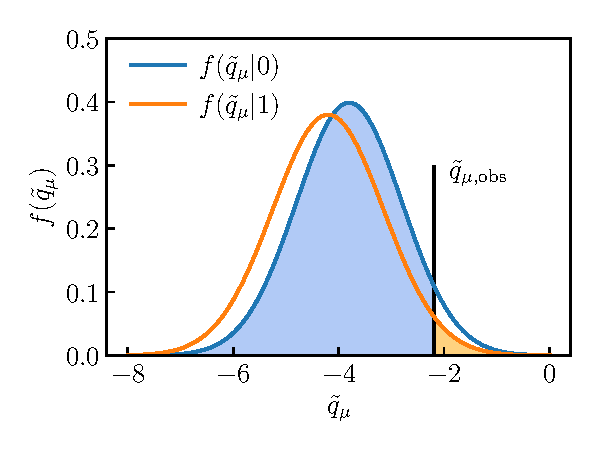
\includegraphics[width=\textwidth]{cls_1}
		\vspace{-1.5em}
		\caption{\label{fig:cls_close}}
	\end{subfigure}\hfill
	\begin{subfigure}[b]{0.47\linewidth}
		\centering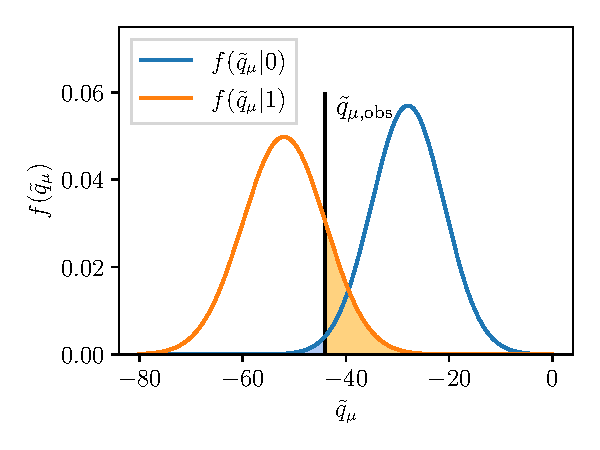
\includegraphics[width=\textwidth]{cls_2}
		\vspace{-1.5em}
		\caption{\label{fig:cls_far}}
	\end{subfigure}%
	\caption{Distribution of the \glspl{pdf} of the signal plus background (in orange) and background-only (in blue) models. The orange and blue coloured areas represent the $p_{s+b}$ and $p_{b}$ values, respectively. Figure~\subref{fig:cls_close} shows a case where both \glspl{pdf} are close together, while figure \subref{fig:cls_close} shows a case where they are well separated. Figures created by the author but based on \reference\cite{Cowan:2013pha}.}\label{fig:cls_method}
\end{figure}

In the CL$_{s+b}$ method, a signal-plus-background model is excluded if $p_{s+b} < \alpha$, where $\alpha$ is defined by the desired confidence level, typically $\mathrm{CL} = 1 - \alpha = 95\%$, and $p_{s+b}$ can be calculated using the test statistic $\tilde{q}_\mu$ (with $\mu = 1$) introduced in~\cref{eq:upper_limit_test_statistic}. If the experiment has very low sensitivity to a specific signal-plus-background model, \eg because the production cross section is too low, the distribution of the test statistic of the signal-plus-background model will be very close to that of the background-only model. In case of an underfluctuation in data, the $\mu = 1$ model can then be falsely excluded, even though no sensitivity is expected. \Cref{fig:cls_method} illustrates this with a simple example. In fact, the exclusion of models to which the experiment has no sensitivity has a probability of at least $\alpha$~\cite{Cowan:2013pha}.

This problem can be remedied by adopting the CL$_s$ method~\cite{Read:2002hq}, altering the threshold for excluding a model in a way to avoid exclusion of models to which the experiment has very low sensitivity. The CL$_s$ value is defined as
\begin{equation}
	\mathrm{CL}_s = \frac{p_{s+b}}{1-p_b},
\end{equation}
where $p_b$ is the $p$-value of the background-only hypothesis\footnote{It is worth highlighting that $p_b$ is equal to $p_\mu$ from \cref{eq:pmu} with $\mu=0$. This is strictly different from $p_0$ in \cref{eq:disc_pvalue} as it relies a different test statistic.}. If the distributions of the test statistics for the signal-plus-background and the background-only models are close to each other (as seen in~\cref{fig:cls_close}) a small value of $p_{s+b}$ due to an underfluctuation in data will entail a large value of $p_b$. Consequently, in the calculation of the CL$_s$ value, $p_{s+b}$ will be penalised by $1-p_b$ (that will be close to 0), resulting in CL$_s > p_{s+b}$, preventing the exclusion of the signal-plus-background model. Conversely, in the case where the two test statistics are well-separated (see~\cref{fig:cls_far}) and $p_{s+b} < \alpha$, then $p_b$ will also be small and thus CL$_s$ will be close to $p_{s+b}$ obtained by the frequentist approach. 

\section{Asimov dataset}

Searches for \gls{bsm} physics are not only interested in the significance obtained using the dataset measured by the experiment, but also in the expected (or median) significance obtained for rejecting different values of $\mu$.
For example, for rejecting the $\mu = 1$ hypothesis, searches are interested in the expected significance obtained assuming data generated according to the $\mu = 0$ hypothesis.

The expected experimental sensitivity can be determined using an artificial dataset called the \textit{Asimov dataset}, defined such that \glspl{mle} of all parameters determined using Asimov data correspond to the true parameter values.
This is achieved by constructing a dataset where the number of events in each bin is exactly equal to the expected event rate in that bin. Using Asimov data, the Asimov likelihood $L_\mathrm{A}$ as well as the profile likelihood $\lambda_\mathrm{A}$ can be evaluated and thus a median significance can be determined.
Non-integer values for data are not an issue as factorial terms from the Poisson probabilities are canceled in the profile likelihood and can thus be dropped altogether. 

\section{Sensitivity estimation}\label{sec:sensitivity_estimation}

When designing search regions for an analysis, it is necessary to achieve an optimal signal-to-background separation power.
A significance metric is needed in order to quantify the separation power and to have a metric to optimise for.
In the following, the expected discovery significance introduced in \reference\cite{Cousins:2007bmb} is used. As the full statistical model is in general not yet known when designing the search regions, appropriate assumptions have to be made. In a \textit{cut-and-count} selection where only the total number of events after a selection are relevant (and not \eg their distribution), the significance is determined by the total number of signal events $S$, the total number of background events $B$ and the uncertainty on the expected number of background events $\Delta B$.
This can be modelled as a so-called \textit{on/off problem}\footnote{The \textit{on/off} nomenclature originates from gamma ray astronomy where \textit{on} refers to the telescope pointing on-source (measuring signal and background photons), while \textit{off} refers to it pointing off-source (measuring only background photons). This problem is an exact analog to the \gls{hep} problem herein, where the off-source measurement typically corresponds to some \textit{sideband} measurement, \ie a measurement of events in a region of a parameter disjoint from the parameter range where the signal might exist.}~\cite{Cousins:2007bmb, Cranmer:2005hi}, where the \textit{cut-and-count} experiment uses two bins, a \gls{sr} enriched in signal events, and a \gls{cr} containing only background events.
In the background-only hypothesis, the parameter $\tau = n_\mathrm{CR} / n_\mathrm{SR}$ then denotes the ratio between the event rate in the \gls{cr}, $n_\mathrm{CR}$, and the event rate in the \gls{sr}, $n_\mathrm{SR}$.

If $\tau$ is known, then the likelihood of this simple configuration can be written in terms of the expected background event rate
\begin{equation}
	L (\mu,B) = \mathrm{Pois}(n_{\mathrm{SR}}\vert\mu S + B) \cdot \mathrm{Pois}(n_{\mathrm{CR}}\vert\tau B),
\end{equation} 
where $\mu$ is again the signal strength parameter. The relative background uncertainty can thus be treated as coming from a Poisson-distributed auxiliary measurement containing only background (\ie in the \gls{cr}) with corresponding uncertainty $\sqrt{\tau B}$, leading to the approximation
\begin{equation}
	\tau = \frac{B}{\Delta B^2}.
\end{equation}
As $n_{\mathrm{SR}}$ and $n_{\mathrm{CR}}$ are each drawn from a Poisson probability with unknown means $\nu_\mathrm{SR}$ and $\nu_\mathrm{CR}$, the background-only hypothesis corresponds exactly to the case where the ratio of Poisson means $\lambda = \nu_\mathrm{CR} / \nu_\mathrm{SR}$ is equal to $\tau$~\cite{Cousins:2007bmb}. The two Poisson terms can then be written as the product of a single Poisson term with mean $n_\mathrm{tot} = n_\mathrm{SR} + n_\mathrm{CR}$ and the binomial probability of picking $n_\mathrm{SR}$ events out of $n_\mathrm{tot}$ with probability $\rho = \nu_\mathrm{SR} / \nu_\mathrm{tot} = 1 / (1+\lambda)$. The likelihood can thus be written as
\begin{equation}
\begin{split}
	L(\mu, B) & = \mathrm{Pois} (n_\mathrm{tot}\vert\lambda_\mathrm{tot})\cdot B(n_\mathrm{SR}\vert\rho,n_\mathrm{tot}) \\ 
	& = \frac{e^{-\lambda_\mathrm{tot}}\lambda_{\mathrm{tot}}^{n_\mathrm{tot}}}{n_\mathrm{tot}\,!} \cdot{n_\mathrm{tot}\choose n_\mathrm{SR}} \rho^\lambda_\mathrm{tot} (1-\rho)^{n_\mathrm{tot}-n_\mathrm{SR}}.
\end{split}
\end{equation}

Since the background-only hypothesis cannot only be expressed as $\mu = 0$ but also as $\nu_\mathrm{SR} = \nu_B$, $\lambda = \tau$, and especially also as $\rho = 1/(1+\tau)$~\cite{Cousins:2007bmb}, its $p$-value can be calculated using the well-know frequentist binomial test,
\begin{equation}
	p_\mathrm{B} = \sum_{j=n_\mathrm{SR}}^{n_\mathrm{tot}} B (j\vert n_\mathrm{tot}, \rho).
\end{equation}
The significance corresponding to $p_\mathrm{B}$ can be derived using~\cref{eq:significance} and is computable in a numerically fast way using the incomplete beta function. The algorithm used for calculating $Z_\mathrm{B}$ in this work is implemented in the \texttt{RooStats::NumberCountingUtils} methods in \textsc{Root}~\cite{ROOT:1997pa,ROOT-2}.



